

\subsection{Opis modela}
Osnovni tipovi entiteta su Klijent i Zaposleni. Specijalizacijom su izvedeni tipovi entiteta Administrator, Vozach, Serviser. Tip entiteta zaposleni povezan je sa tipom entiteta Sektor preko stranog kljucha, a koji chuva podatke o ulogama zaposlenih i sektorima u kojima rade (administrator, vozach, serviser...). Tip entiteta Vozilo chuva podatke o vozilima. Tip entiteta Obrada prijave kvara nastao je agregacijom tipova entiteta Vozach i Vozilo i chuva podatke o prijavi kvara vozila. Tip entiteta Magacin chuva podatke o svim aktivnim magacinima klijenata i povezan je sa tipom entiteta Klijent preko stranog kljucha.

Poshto je za pravilno funkcionisanje sistema potrebno isposhtovati integritet podataka, predlog je da se koristi relaciona baza podataka.

Na slici \ref{fig:er} se nalazi detaljan logichki model baze podataka. Dakle, dodate su i informacije o kljuchevima, kao i tipovima atributa. 

\begin{figure}[H]
    \centering
    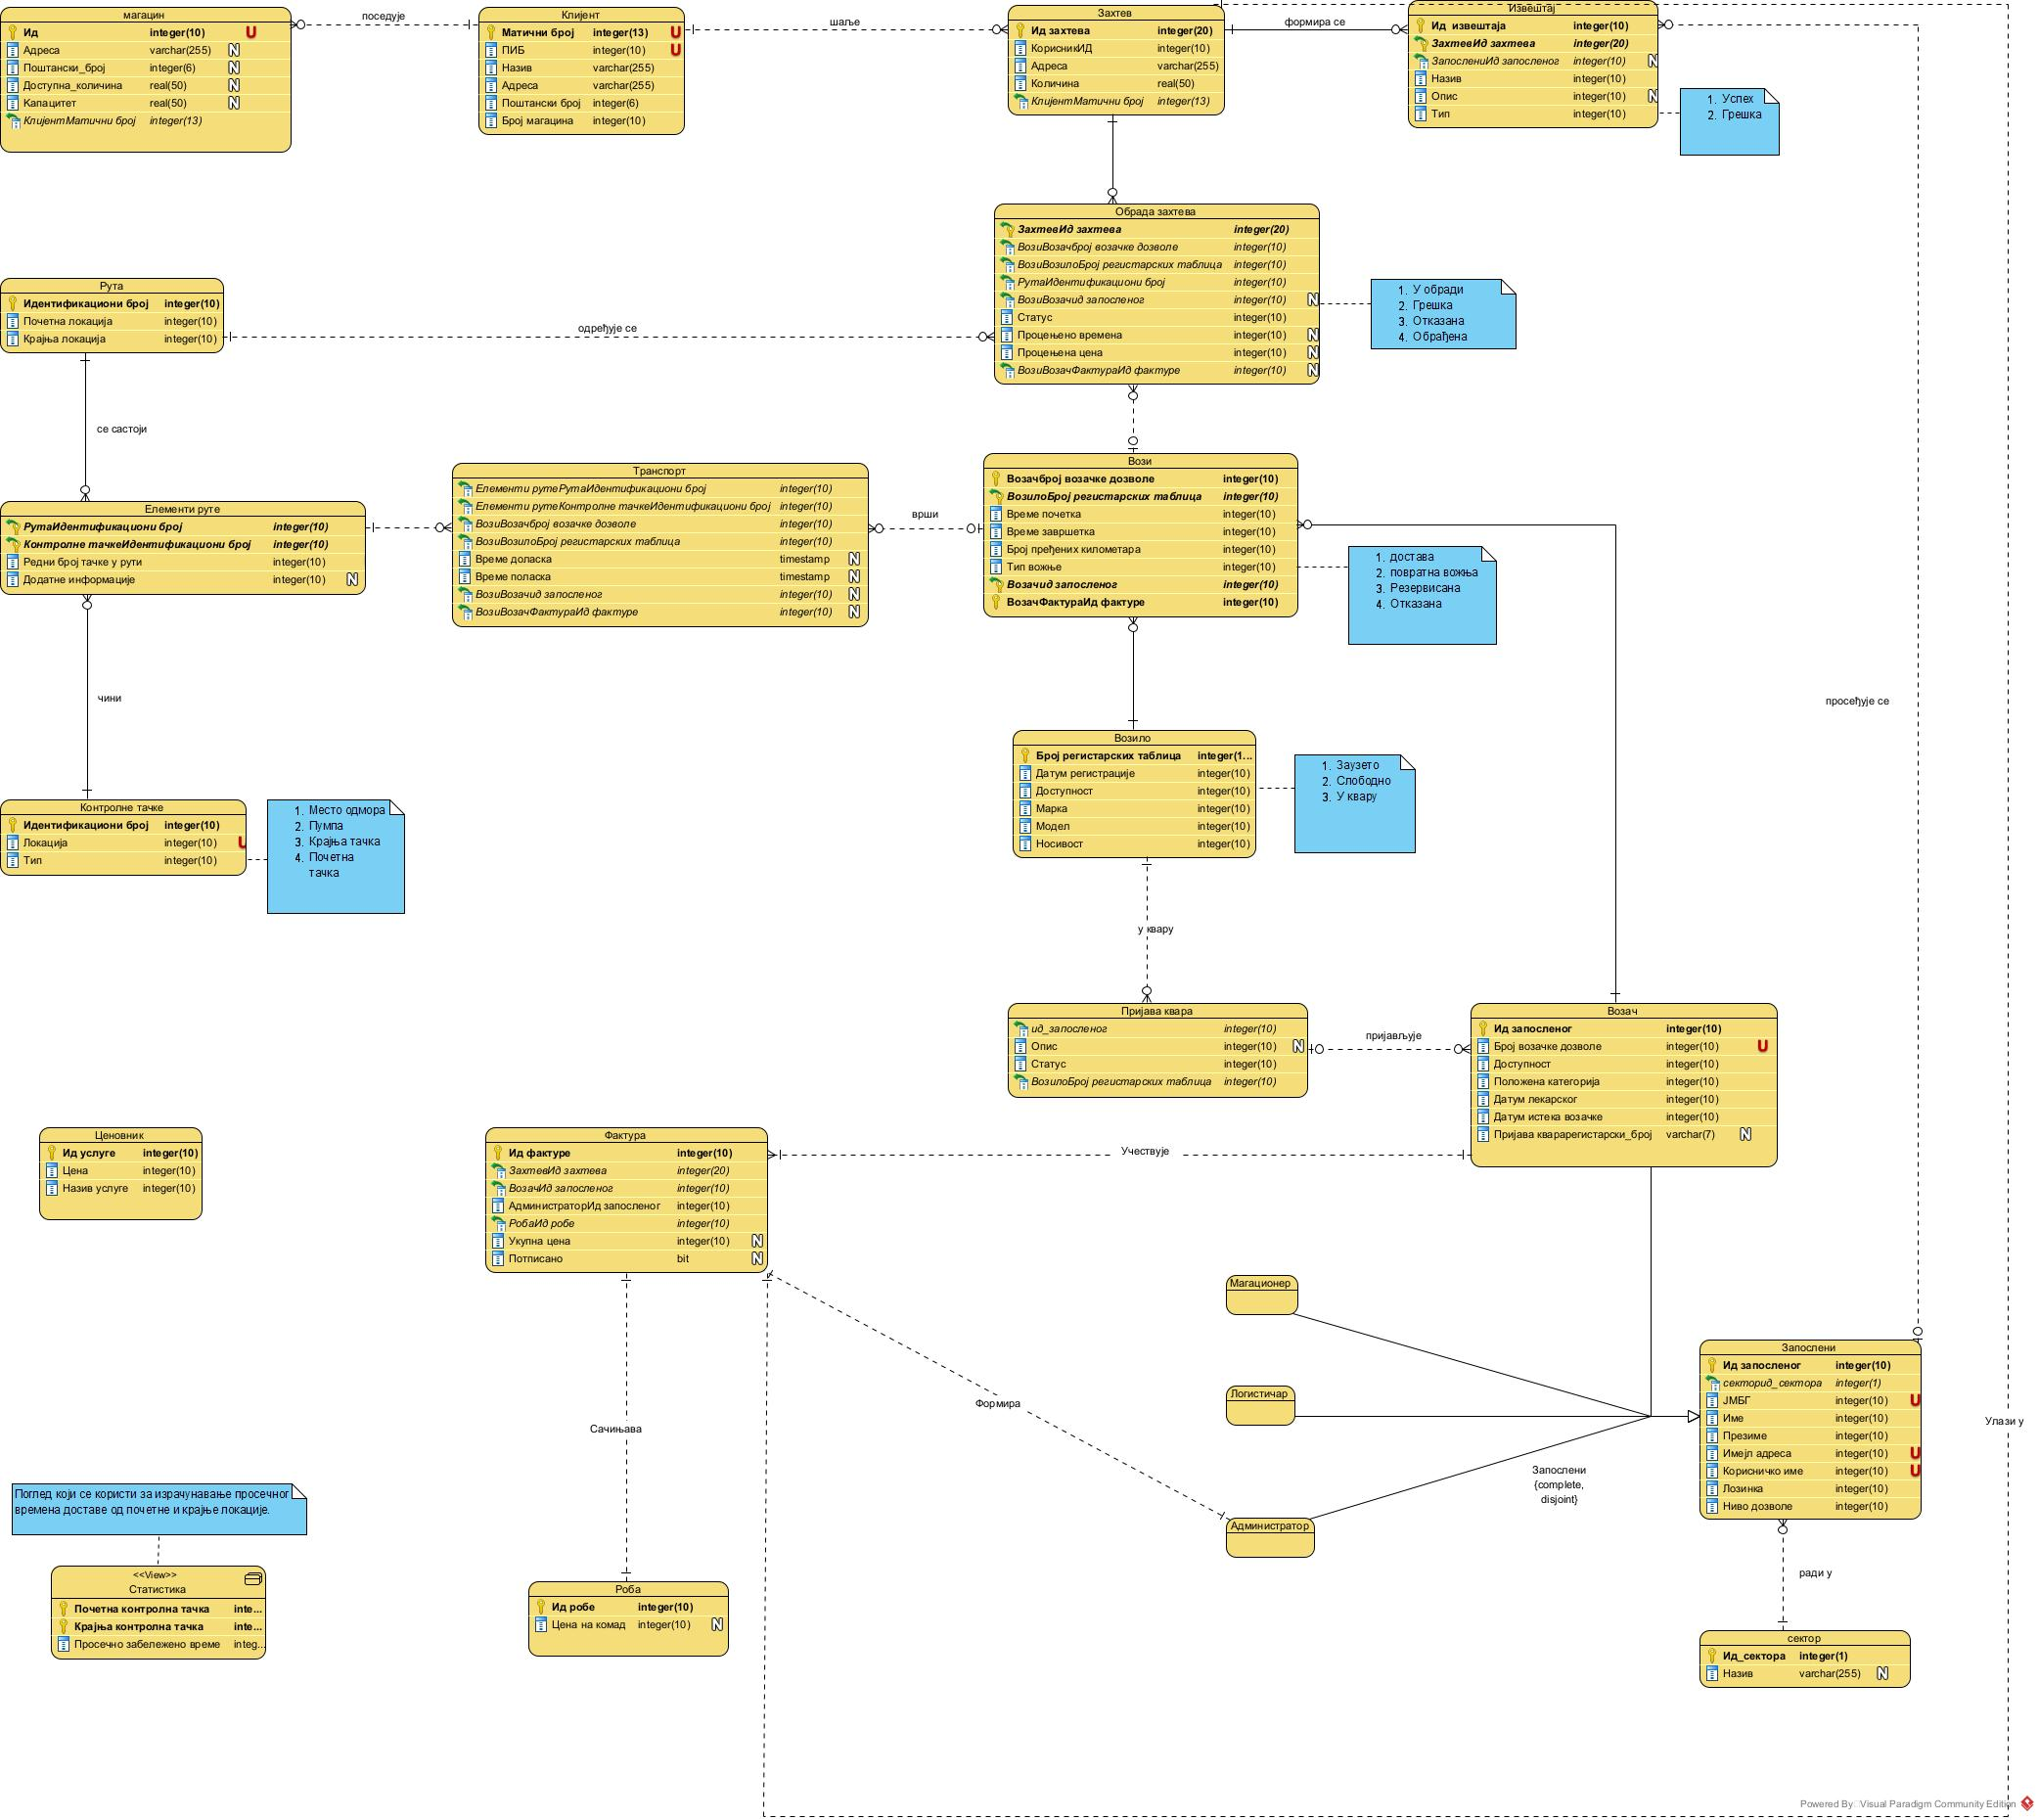
\includegraphics[width=12cm]{Slike/ER.jpg}
    \caption{Dijagram objekti-veze baze podataka}
    \label{fig:er}
\end{figure}
\newpage
\begin{itemize}
    \item 



Atributi tipa entiteta Klijent su:
\begin{enumerate}
    \item{matichni broj (PK, niz intid2era duz1ine 8)}
    \item{pib (niz intid2era duz1ine 10)}
    \item{naziv (niz karaktera duz1ine 255)}
    \item{adresa (niz karaktera duz1ine 255)}
    \item{poshtanski broj (intid2er)}
    \item{broj aktivnih magacina (intid2er)}
\end{enumerate}

\item
Atributi tipa entiteta Magacin su:
\begin{enumerate}
    \item{id (PK, intid2er)}
    \item{matichni broj (SK, niz intid2era duz1ine 8)}
    \item{adresa (niz karaktera duz1ine 255)}
    \item{poshtanski broj (intid2er)}
    \item{dostupna kolichina (intid2er)}
    \item{kapacitet (intid2er)}
\end{enumerate}
\item
Atributi tipa entiteta Zaposleni:
\begin{enumerate}
    \item {id zaposlenog (PK, intid2er)}
    \item{JMBG (niz intid2era duz1ine 13)}
    \item{ime (niz karaktera duz1ine 255)}
    \item{prezime (niz karaktera duz1ine 255)}
    \item{imejl adresa (niz karaktera duz1ine 255)}
    \item{korisnichko ime (niz karaktera duz1ne 255)}
    \item{lozinka (niz karaktera duz1ne 255)}
    \item{id sektora (SK, intid2er)}
    \item{nivo dozvola}
\end{enumerate}
\item
Atributi tipa entiteta Vozach:
\begin{enumerate}
    \item {id zaposlenog (PK/SK, intid2er)}
    \item{broj vozache dozvole (intid2er)}
    \item{dostupnost (dostupan/zauzet)}
    \item{poloz1ena kategorija (niz karaktera duz1ine 6)}
    \item{datum lekarskog (datum)}
    \item{datum isteka vozachke (datum)}
\end{enumerate}
\item
Atributi tipa entiteta Sektor:
\begin{enumerate}
    \item {id sektora (PK, intid2er)}
    \item{naziv (niz karaktera duz1ine 255)}
\end{enumerate}
\item
Atributi tipa entiteta Vozilo:
\begin{enumerate}
    \item {broj registarskih tablica (PK, niz karaktera duz1ine 7)}
    \item{datum registracije (datum)}
    \item{dostupnost (zauzeto/slobodno/u kvaru)}
    \item{marka (niz karaktera duz1ne 255)}
    \item{model (niz karaktera duz1ine 255)}
    \item{nosivost (intid2er)}
\end{enumerate}
\item
Agregirani tip entiteta Obrada prijave kvara:
\begin{enumerate}
    \item {id zaposlenog (PK/SK, intid2er)}
    \item{broj registarskih tablica (PK/SK, niz karaktera duz1ne 7)}
    \item{opis (niz karaktera duz1ine 255)}
    \item{status (u kvaru/popravka/popravljeno)}
\end{enumerate}

\item Entitet cenovnik
    \begin{itemize}
        \item Neophodan entitet u modelu baze podataka, u kome se chuvaju informacije o ceni prevoza.
        \item U ovom odeljku c1e biti detaljno opisan i nachin rachunanja cene troshkova. 
        Varijabilni troshkovi su direktni troshkovi povezani sa vozhnjom svakog kilometara. Ovi troshkovi se povec1avaju i smanjuju na osnovu broja kilometara koji se pređu u datom mesecu. Na primer, gorivo je promenljivi troshak. Morate da kupite gorivo za svaki kilometar koji pređete. Pored goriva, varijabilni troshkovi su i obroci, telefon, gume, odrzhavanje i tako dalje.
Kada je u pitanju nasha kompanija rachunica zbirnog transporta je veoma jednostavna i rachuna se po zapremini i težini.
Rachunanje se vrshi po tome koliko kilograma korisnog tovara chini poshiljka.  
Ono što je posebno bitno je to što za klijenta sigurno nec1e biti 
 neprijatnih iznenadenja i iznenadnih troškova. 
    \end{itemize}
\item Pogled Statistika
    \begin{itemize}
        \item Nash sistem korisniku nakon obrade zahteva shalje i procenu vremena dostave. Ova informacija se dobija iz baze podataka, uz pomoc1 pogleda Statistika, gde se chuvaju sve informacije o vremenu transporta izmed1u dve kontrolne tachke. Prosechno vreme nam dobijamo usrednjavanjem vremena izmed1u svih tachki rute.
        Odlucheno je da se modeluje kao pogled, da bi se uvek radilo sa najazhurnijim podacima.

        
        
    \end{itemize}

\end{itemize}



\subsection{Privilegije korisnika}
Sa obzirom na to da sistemu pristupaju razlichiti korisnici, potrebno je prodiskutovati i privilegije koje svaki od njih ima nad bazom podataka prilikom pristupa sistemu i koje je potrebno isposhtovati prilikom fizichke implementacije baze podataka.

\begin{enumerate}
    \item Korisnici, Vozachi i Magacioneri imaju samo privilegije chitanja.
    \item Logistichari mogu da menjaju odredjene informacije vezane za planiranje transporta. Dakle, mogu da dodaju/brishu kljuchne tachke rute, kao i samu rutu, kao i informacije o zahtevu i njegovoj obradi. Ostale informacije mogu samo da chitaju.

    \item Administratori imaju privilegije chitanja, pisanja i menjanja svih informacija.

\end{enumerate}

% Број регистарских таблица	integer	10	true	false	false
% Датум регистрације	integer	10	false	false	false
% Доступност	integer	10	false	false	false
% Марка	integer	10	false	false	false
% Модел	integer	10	false	false	false
% Носивост	integer	10	false	false	false